
%=========================================================
	El sistema se encuentra organizado por módulos con la finalidad de agrupar y administrar de mejor manera los requerimientos funcionales del sistema. Dividir el sistema en módulos permite visualizar e identificar rápidamente aquellos aspectos funcionales que pueden tratarse conjuntamente. \\

    Las figuras \ref{fig:ModulosWeb} y \ref{fig:ModulosMovil} muestran los módulos propuestos de manera inicial para la aplicación \textbf{Conexión iE}. Cada uno de estos módulos agrupan los casos de uso que poseen funcionalidad similar o que trabajan en conjunto para alcanzar un aspecto funcional del sistema. Cada uno de los módulos que se muestran en la figura se describen a continuación:

%    La figura \ref{fig:ModulosPAEAR} muestra los módulos que conforman el \saear. Cada uno de estos módulos agrupan los casos de uso que poseen funcionalidad similar o que trabajan en conjunto para alcanzar un aspecto funcional del sistema. Cada uno de los módulos que se muestran en la figura se describen a continuación:

    \begin{figure}[h!]
	\begin{center}
	      \fbox{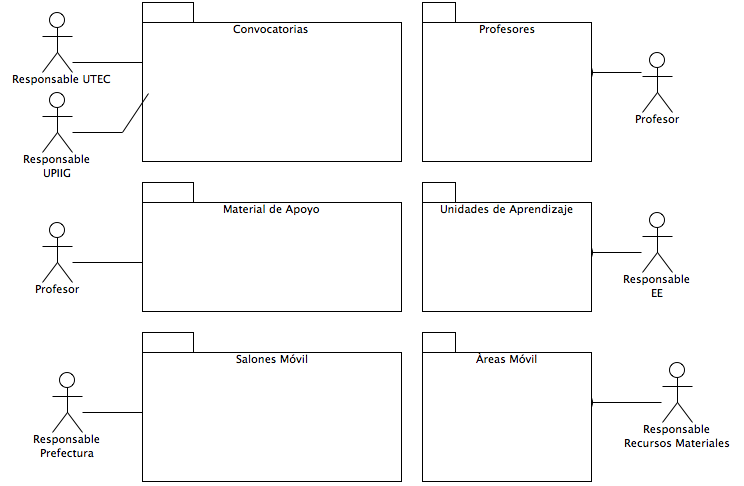
\includegraphics[width=\textwidth]{images/modulos.png}}
	\caption{Módulos Web de la Aplicación Conexión iE.}
	\label{fig:ModulosWeb}
	\end{center}
    \end{figure}

    \begin{figure}[h!]
	\begin{center}
		\fbox{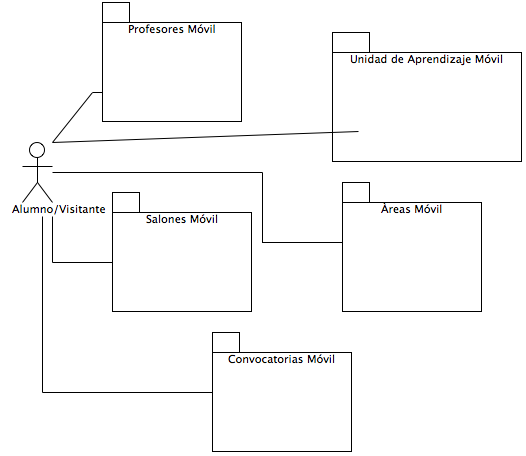
\includegraphics[width=\textwidth]{images/modulosmovil.png}}
		\caption{Módulos Móvil de la Aplicación Conexión iE.}
		\label{fig:ModulosMovil}
	\end{center}
\end{figure}


    \begin{itemize}
	\item {\bf Salones:} Este módulo agrupa los casos de plataforma web  que se relacionan con los salones que pertenecen a la Escuela Superior de Cómputo y al encargado de prefectura, es decir:
	\begin{itemize}
		\item Gestionar Salón.
		\item Registrar de Salón.
		\item Editar Salón.
		\item Eliminar Salón.
		\item Consultar Salón.
	\end{itemize}

  
	\item {\bf Áreas:} Este módulo agrupa los casos de plataforma web  que se relacionan con las áreas que pertenecen a la Escuela Superior de Cómputo, es decir:
	\begin{itemize}
		\item Gestionar Áreas.
		\item Registrar de Áreas.
		\item Editar Áreas.
		\item Eliminar Áreas.
		\item Consultar Áreas.
	\end{itemize}

	\item {\bf Salones Móvil:} Este módulo agrupa los caso de uso de plataforma móvil que se realcionan con los salones pertenecientes a la Escuela Superior de Cómputo y al alumno, es decir:
		\begin{itemize}
			\item Consultar Asignación de Grupos.
			\item Consultar Nivel de Salón.
			\item Consultar Edifcio de Salón.
		\end{itemize}

	\item {\bf Áreas Móvil:} Este módulo agrupa el caso de uso de plataforma móvil que se realcionan con lass principales áreas pertenecientes a la Escuela Superior de Cómputo y al alumno, es decir:
	\begin{itemize}
		\item Consultar Área.
	\end{itemize}

	\item {\bf Profesores:} Este móduulo agrupa los casos de uso de plataforma web que proporcionan información sobre la consulta de profesores que pertenecen a la Escuela Superior de Cómputo, tales como:
	\begin{itemize}
		\item Registrar Profesor.
		\item Editar Profesor.
		\item Eliminar Profesor.
		\item Consultar Profesor.
	\end{itemize} 

	\item {\bf Profesores Móvil:} Este móduulo agrupa los casos de uso de plataforma móvil que proporcionan información sobre la consulta de profesores que pertenecen a la Escuela Superior de Cómputo, tales como:
\begin{itemize}
	\item Consultar Profesor.
	\item Consultar Detalle de Profesor.
\end{itemize} 

\item {\bf Material de Apoyo:} Este módulo agrupa los casos de plataforma web  que se relacionan con el material de apoyo las unidades de aprendizaje que imparten los profesoresen la Escuela Superior de Cómputo y al encargado de prefectura, es decir:
\begin{itemize}
	\item Gestionar Material de Apoyo.
	\item Registrar Material de Apoyo.
	\item Editar Material de Apoyo.
	\item Eliminar Material de Apoyo.
	\item Consultar Material de Apoyo.
\end{itemize}

	\item {\bf Unidades de Aprendizaje Móvil:} Este módulo agrupa los caso de uso de plataforma móvil que se realcionan con los salones pertenecientes a la Escuela Superior de Cómputo y al alumno, es decir:
\begin{itemize}
	\item Consultar Unidades de Aprendizaje.
	\item Consultar Material de Apoyo
	\item Consultar Detalle de Unidades de Aprendizaje.
	\item Consultar Programa Académico de Unidad de Aprendizaje.
\end{itemize}

	\item {\bf Unidades de Aprendizaje:} Este módulo agrupa los casos de plataforma web  que se relacionan con las unidades de aprendizaje que se imparten por semesntre en la Escuela Superior de Cómputo y al encargado de prefectura, es decir:
\begin{itemize}
	\item Gestionar Unidad de Aprendizaje.
	\item Registrar Unidad de Aprendizaje.
	\item Editar Unidad de Aprendizaje.
	\item Eliminar Unidad de Aprendizaje.
	\item Consultar Unidad de Aprendizaje.
\end{itemize}

\item {\bf Convocatorias:} Este módulo agrupa los casos de plataforma web  que se relacionan con las las convocatorias que se ofertan por semesntre en la Escuela Superior de Cómputo, es decir:
\begin{itemize}
	\item Gestionar Convocatoria.
	\item Registrar Convocatoria Cursos.
	\item Editar Convocatoria Cursos.
	\item Eliminar Convocatoria Cursos.
	\item Consultar Convocatoria Cursos.
	\item Registrar Convocatoria Movilidad.
	\item Editar Convocatoria Movilidad.
	\item Eliminar Convocatoria Movilidad.
	\item Consultar Convocatoria Movilidad.
\end{itemize}

	\item {\bf Convocatoria Móvil:} Este móduulo agrupa los casos de uso de plataforma móvil que proporcionan información sobre las convocatorias ofrecidas en la Escuela Superior de Cómputo, tales como:
\begin{itemize}
	\item Consultar Convocatoria.
	\item Consultar Convocatoria Cursos.
	\item Consultar Convocatoria Movilidad.
		\item Consultar Convocatoria Nacional.
			\item Consultar Convocatoria Internacional.
\end{itemize}
%	\item {\bf Administración de usuarios:} Integra los casos de uso referentes a la administración de los usuarios y al control de acceso al sistema.

	%El presente documento expone en detalle la información correspondiente al módulo de \textbf{Registro de escuelas}.

    \end{itemize}

%=========================================================
\section{Actores del sistema}\label{sec:Comportamiento:ActoresSistema}

Los actores son los perfiles asociados a las diversas áreas que intervienen en el proceso. Se han identificado los actores de acuerdo a las actividades y responsabilidades dentro de la aplicación \textbf{Conexión iE}, los cuales se muestran en la figura \ref{fig:perfilesWeb} y se describen a continuación.

%    Los actores son los perfiles asociados a las diversas áreas y/u organizaciones que intervienen en el proceso. Se han identificado los actores de acuerdo a las actividades y responsabilidades dentro del \paear respecto al módulo de \textbf{Registro de escuelas}, los cuales se muestran en la figura \ref{fig:perfilesPAEAR} y se describen a continuación. 
    %y responsabilidades dentro del \paear - \saear, los cuales se describen a continuación.

    \begin{figure}[h!]
      \begin{center}
	  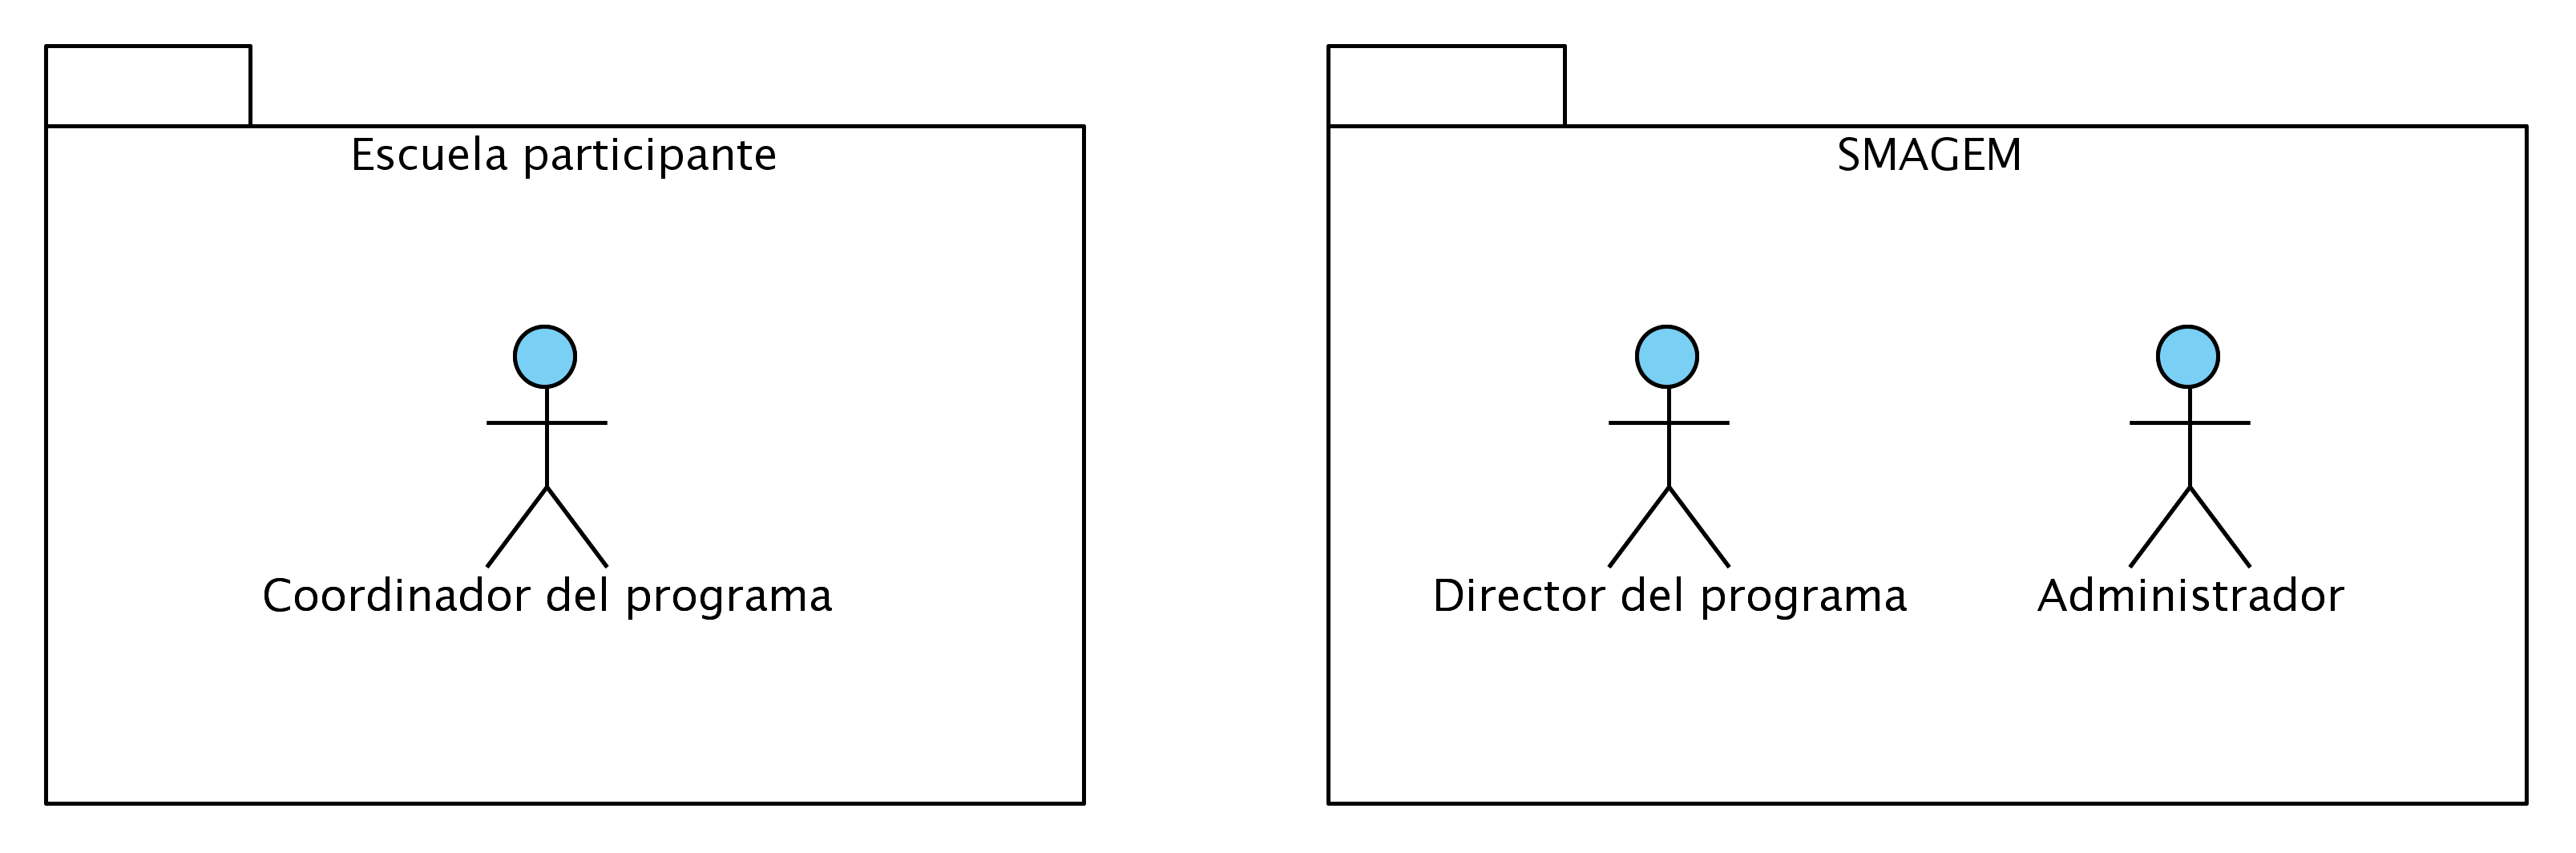
\includegraphics[width=0.6\textwidth]{images/actores/Actores.png}
      \caption{Perfiles identificados.}
      \label{fig:perfilesWeb}
      \end{center}
    \end{figure}

    \begin{figure}[h!]
	\begin{center}
		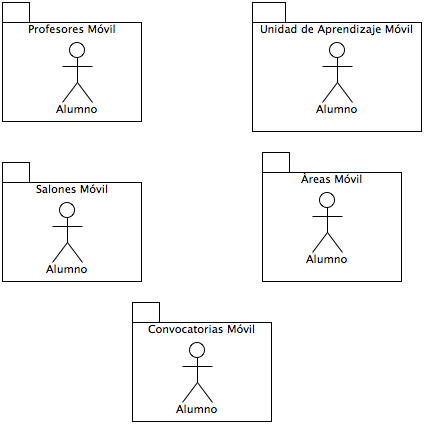
\includegraphics[width=0.6\textwidth]{images/actores/Actoresmovil.png}
		\caption{Perfiles identificados.}
		\label{fig:perfilesMovil}
	\end{center}
\end{figure}
%--------------------------------------------------------------------------------------------------
    \begin{actor}{Alumno}{CIEAlumno}{Persona inscrita dentro del Instituto Politécnico Nacional que solicitará las consultas de espacios, salones asignados a grupos, información sobre los trámites de la escuela y sobre el material de apoyo de las unidades de aprendizaje.}

	\item[Área:] Escuela Superior de Cómputo.

	\item[Responsabilidades:] \hspace{1pt}
	
		\begin{itemize}

		    \item Solicitar la consulta de espacios.
		    \item Solicitar la consulta de salones asignados a grupos.
		    \item Solicitar la consulta de trámites.
		    \item Solicitar la consulta de material de apoyo.
		\end{itemize}


	\item[Perfil:] \hspace{1pt}
		\begin{itemize}
		    \item Ser una persona inscrita en alguna escuela del Instituto.
		    \item Tener conocimiento de las últimas tecnologías.
		    \item Conocer la disponibilidad de descarga de la aplicación.
		    \item Contar con un dispositivo iOS.
	    \end{itemize}

	\item[Cantidad:] \textit{N} personas por escuela participante.

\end{actor}

%--------------------------------------------------------------------------------------------------
\begin{actor}{Visitante}{CIEVisitante}{Persona externa al Instituto que desee localizar algún espacio o profesor para asesorías de investigación, consultas de especialidad para tésis, trámites, etc.}

    \item[Área:] Escuela participante.
    \item[Responsabilidades:] \hspace{1pt}

	\begin{itemize}

		  \item Consultar los distintos espacios disponibles en la escuela.
		  \item Consultar la disponibilidad de horario y ubicación de la plantilla docente.
	  
    \end{itemize}

    \item[Perfil:] \hspace{1pt}

	\begin{itemize}

	    \item Conocimientos sobre los temas de interés en investigación de la escuela en cuestión.
	    \item Contar de las tecnologías móviles actuales.
	    \item Conocimientos de la aplicación disponible.

	\end{itemize}

    \item[Cantidad:] \textit{N} por escuela.

\end{actor}

%--------------------------------------------------------------------------------------------------
\begin{actor}{Profesor}{CIEProfesor}{Persona perteneciente al Instituto con responsabilidades académicas y adminstrativas que cuente con su información pública de contacto para su consulta.}
	
	\item[Área:] Escuela participante.
	\item[Responsabilidades:] \hspace{1pt}
	
	\begin{itemize}
		
		\item Proporcionar sus horarios de clase y atención a alumnos.
		\item Proporcionar fotografía y teléfono de contacto si así lo desea.
		\item Proporcionar áreas de interés.
		\item Actualizar horario cada semestre.
		\item Proporcionar material de apoyo para las unidades de apendizaje.
		
	\end{itemize}
	
	\item[Perfil:] \hspace{1pt}
	
	\begin{itemize}
		
		\item Conocimientos sobre los temas de interés en investigación de la escuela en cuestión.
		\item Conocimientos de las tecnologías utlizadas actualmente como medio de difusión y comunicación.
		\item Conocimientos de la aplicación disponible.
		
	\end{itemize}
	
	\item[Cantidad:] \textit{N} por escuela.
	
\end{actor}

%--------------------------------------------------------------------------------------------------
\begin{actor}{Responsable UTEC}{CIEUtec}{Persona perteneciente al Instituto encargada de mantener la información de la Escuela disponible para su consuta, esto involucra trámites, convocatorias, boletín de noticias, etc.}
	
	\item[Área:] Escuela participante.
	\item[Responsabilidades:] \hspace{1pt}
	
	\begin{itemize}
		
		\item Proporcionar la información que se tenga para convocatorias y diversos trámites dentro de la Escuela.
		\item Proporcionar información para el boletín de noticias.
		\item Mantener actualizada la información.

		
	\end{itemize}
	
	\item[Perfil:] \hspace{1pt}
	
	\begin{itemize}
		
		\item Tener conocimiento sobre tecnologías WEB.
		\item Conocimientos de las tecnologías utlizadas actualmente como medio de difusión y comunicación.
		\item Conocimientos de la aplicación móviles.
		\item Conocimientos sobre la disponibilidad de la aplicación.	
	\end{itemize}
	
	\item[Cantidad:] Una persona por escuela.
	
\end{actor}

%--------------------------------------------------------------------------------------------------
\begin{actor}{Responsable UPIIG}{CIEUpiig}{Persona perteneciente al Instituto }
	
	\item[Área:] Escuela participante.
	\item[Responsabilidades:] \hspace{1pt}
	
	\begin{itemize}
		
		\item Proporcionar la información que se tenga para convocatorias y diversos trámites dentro de la Escuela.
		\item Proporcionar información para el boletín de noticias.
		\item Mantener actualizada la información.
		
		
	\end{itemize}
	
	\item[Perfil:] \hspace{1pt}
	
	\begin{itemize}
		
		\item Tener conocimiento sobre tecnologías WEB.
		\item Conocimientos de las tecnologías utlizadas actualmente como medio de difusión y comunicación.
		\item Conocimientos de la aplicación móviles.
		\item Conocimientos sobre la disponibilidad de la aplicación.	
	\end{itemize}
	
	\item[Cantidad:] Una persona por escuela.
	
\end{actor}
%\begin{actor}{Administrador}{administrador}{Persona encargada de administrar y dar soporte técnico al sistema.}
%
%    \item[Área:] SMAGEM.
%
%    \item[Responsabilidades:] \hspace{1pt}
%
%	\begin{itemize}
%
%	  \item Dar soporte técnico al sistema en lo referente a conectividad y acceso por parte de los usuarios.
%    %\item Puede realizar todas las operaciones de los demás usuarios por instrucciones del Director del Programa.
%
%	\end{itemize}
%
%    \item[Perfil:] \hspace{1pt}
%
%      \begin{itemize}
%
%	\item Conocimientos técnicos y de operación del sistema.
%	\item Conocimientos del sistema operativo sobre el cual se instale el sistema.
%	\item Conocimientos acerca de la administración de sistemas.
%	\item Contar con una cuenta de correo electrónico.
%
%      \end{itemize}
%
%    \item[Cantidad:] Uno para la SMAGEM.
%
%\end{actor}


%====================================================================================
\section{Casos de Uso del módulo de Salones}

    La figura \ref{fig:casosUso:web} muestra los casos de uso que integran la funcionalidad del módulo de Salones, que se refieren a la consulta de edificios, niveles y salones de una ecuela.

    \begin{figure}[h!]
	\begin{center}
	    \fbox{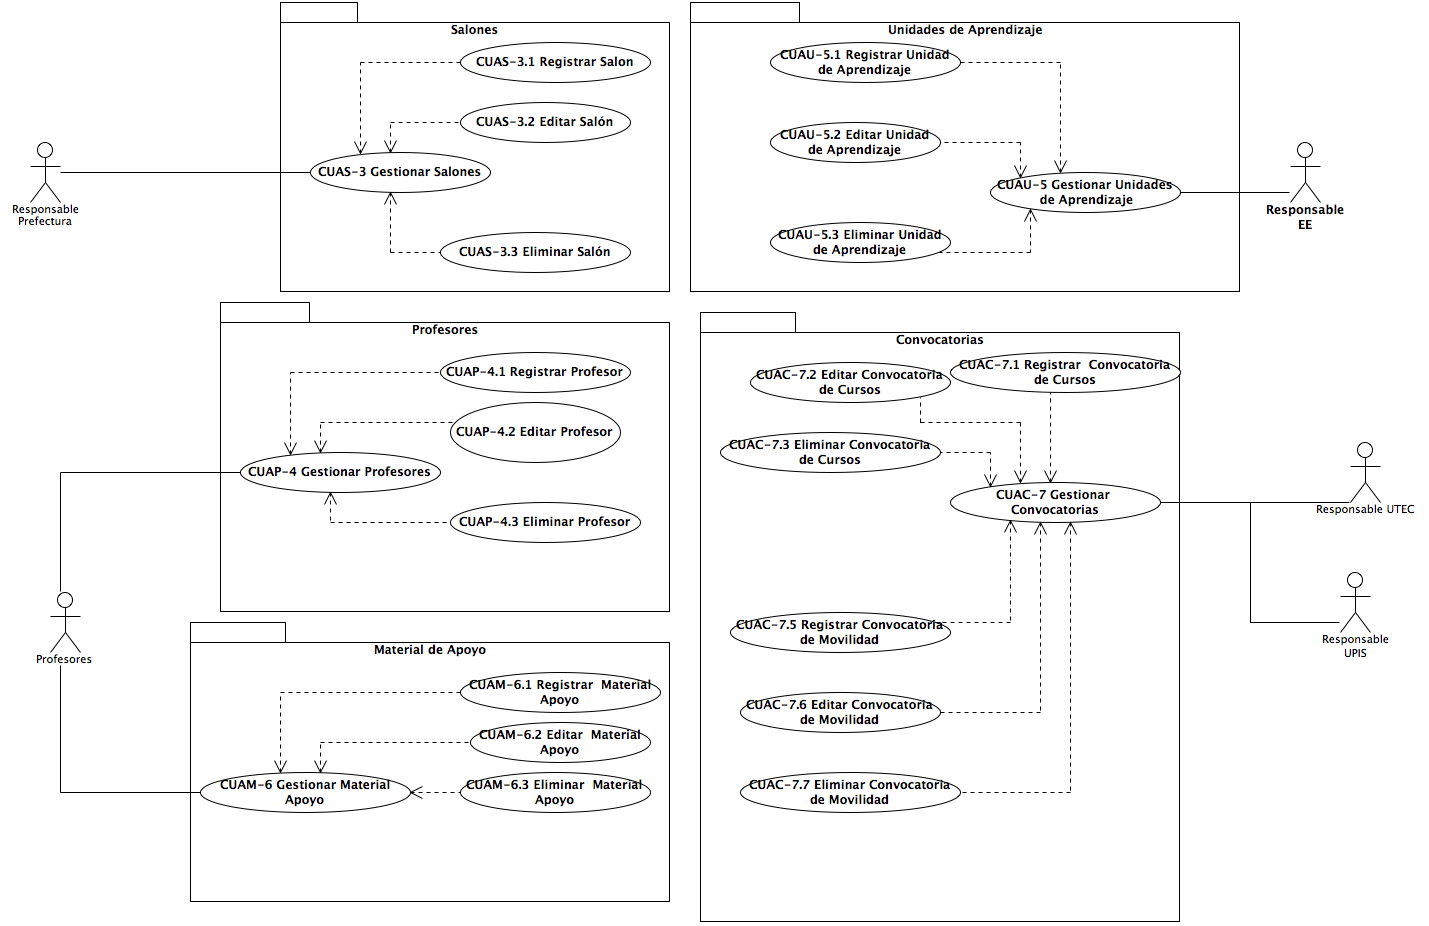
\includegraphics[width=.9\textwidth]{images/CasosUso/cuweb.png}}
	\caption{Diagrama de casos de uso de la aplicación conexión iE Web. \label{fig:casosUso:web}}
	\end{center}
    \end{figure}

\section{Casos de Uso del módulo de Profesores}
La figura \ref{fig:casosUso:movil} muestra los casos de uso que integran la funcionalidad necesaria para la obtención de la información para la ubicación física del cubículo y oficina de un profesor así como la información de contacto institucional y si lo desea, personal.

 \begin{figure}[h!]
     \begin{center}
         \fbox{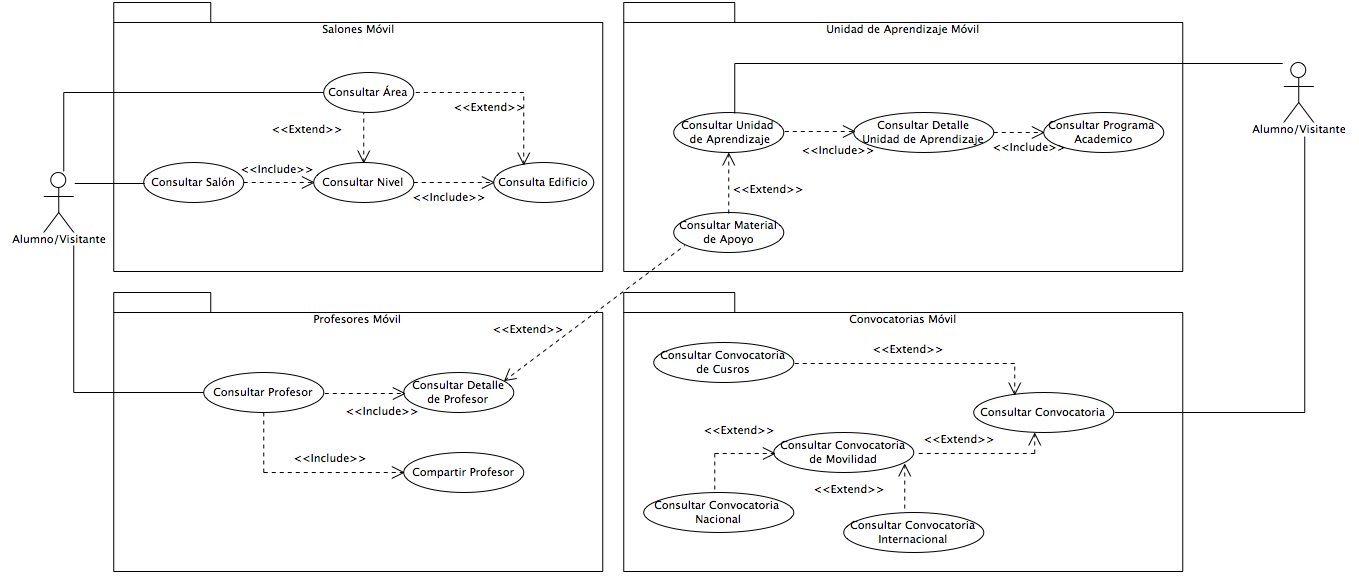
\includegraphics[angle=90, height=0.9\textheight]{images/CasosUso/cumovil.png}}
     \caption{Diagrama de casos de uso para el módulo de Información base para indicadores.}
     \label{fig:casosUso:movil}
     \end{center}
 \end{figure}

%\section{Casos de Uso del módulo de Plan de acción}
%La figura \ref{fig:casosUso:plan} muestra los casos de uso que integran la funcionalidad del módulo de Plan de acción, los cuales permiten el registro y modificación del plan de acción de la escuela. 
%
%\begin{figure}[h!]
%    \begin{center}
%        \fbox{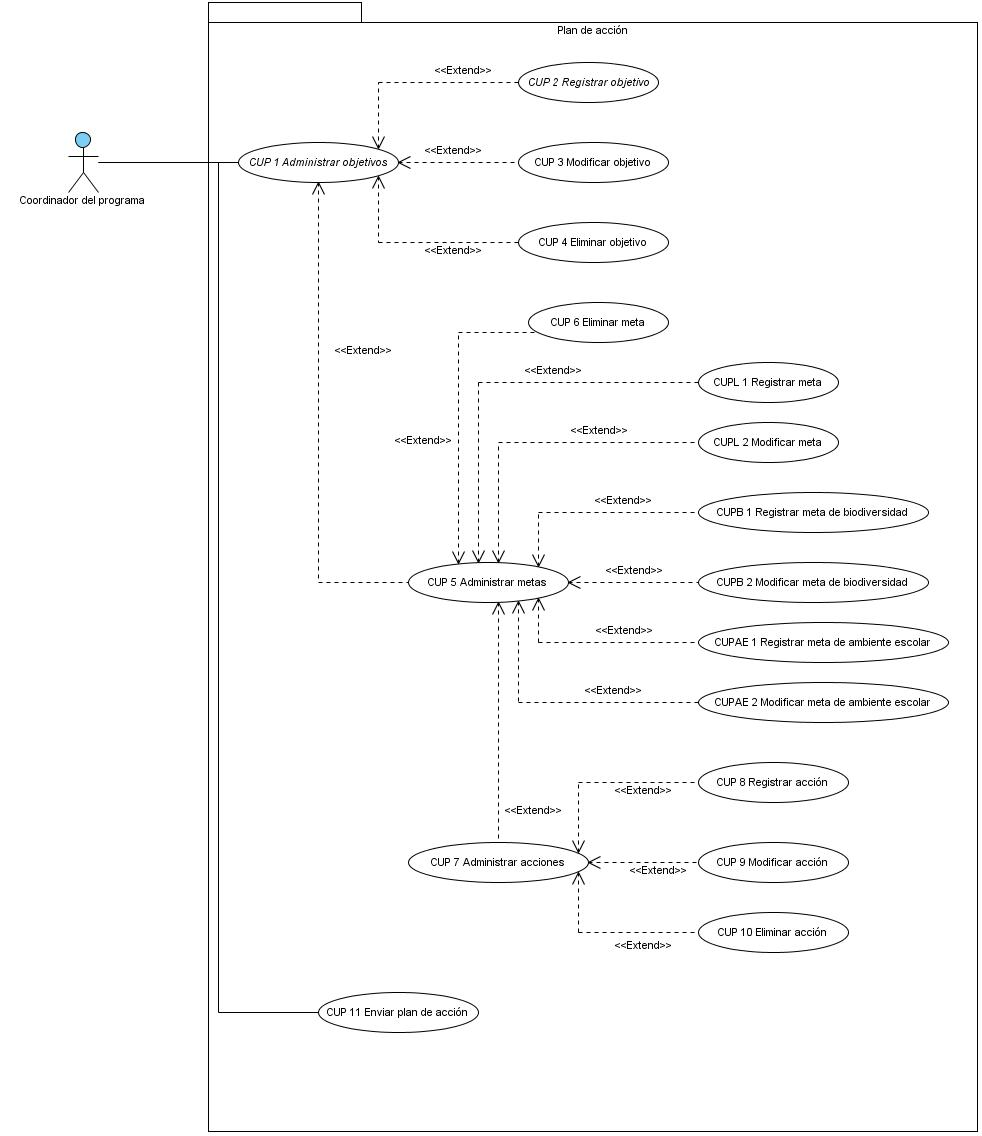
\includegraphics[width=\textwidth]{images/CasosUso/plan.jpg}}
%    \caption{Diagrama de casos de uso para el módulo de Plan de acción.}
%    \label{fig:casosUso:plan}
%    \end{center}
%\end{figure}
%
%\section{Casos de Uso del módulo de Seguimiento y acreditación}
%La figura \ref{fig:casosUso:seguimiento} muestra los casos de uso que integran la funcionalidad del módulo de Seguimiento y acreditación, los cuales permiten el registro y modificación de los avances realizados en el plan de acción de la escuela. 
%
%\begin{figure}[h!]
%    \begin{center}
%        \fbox{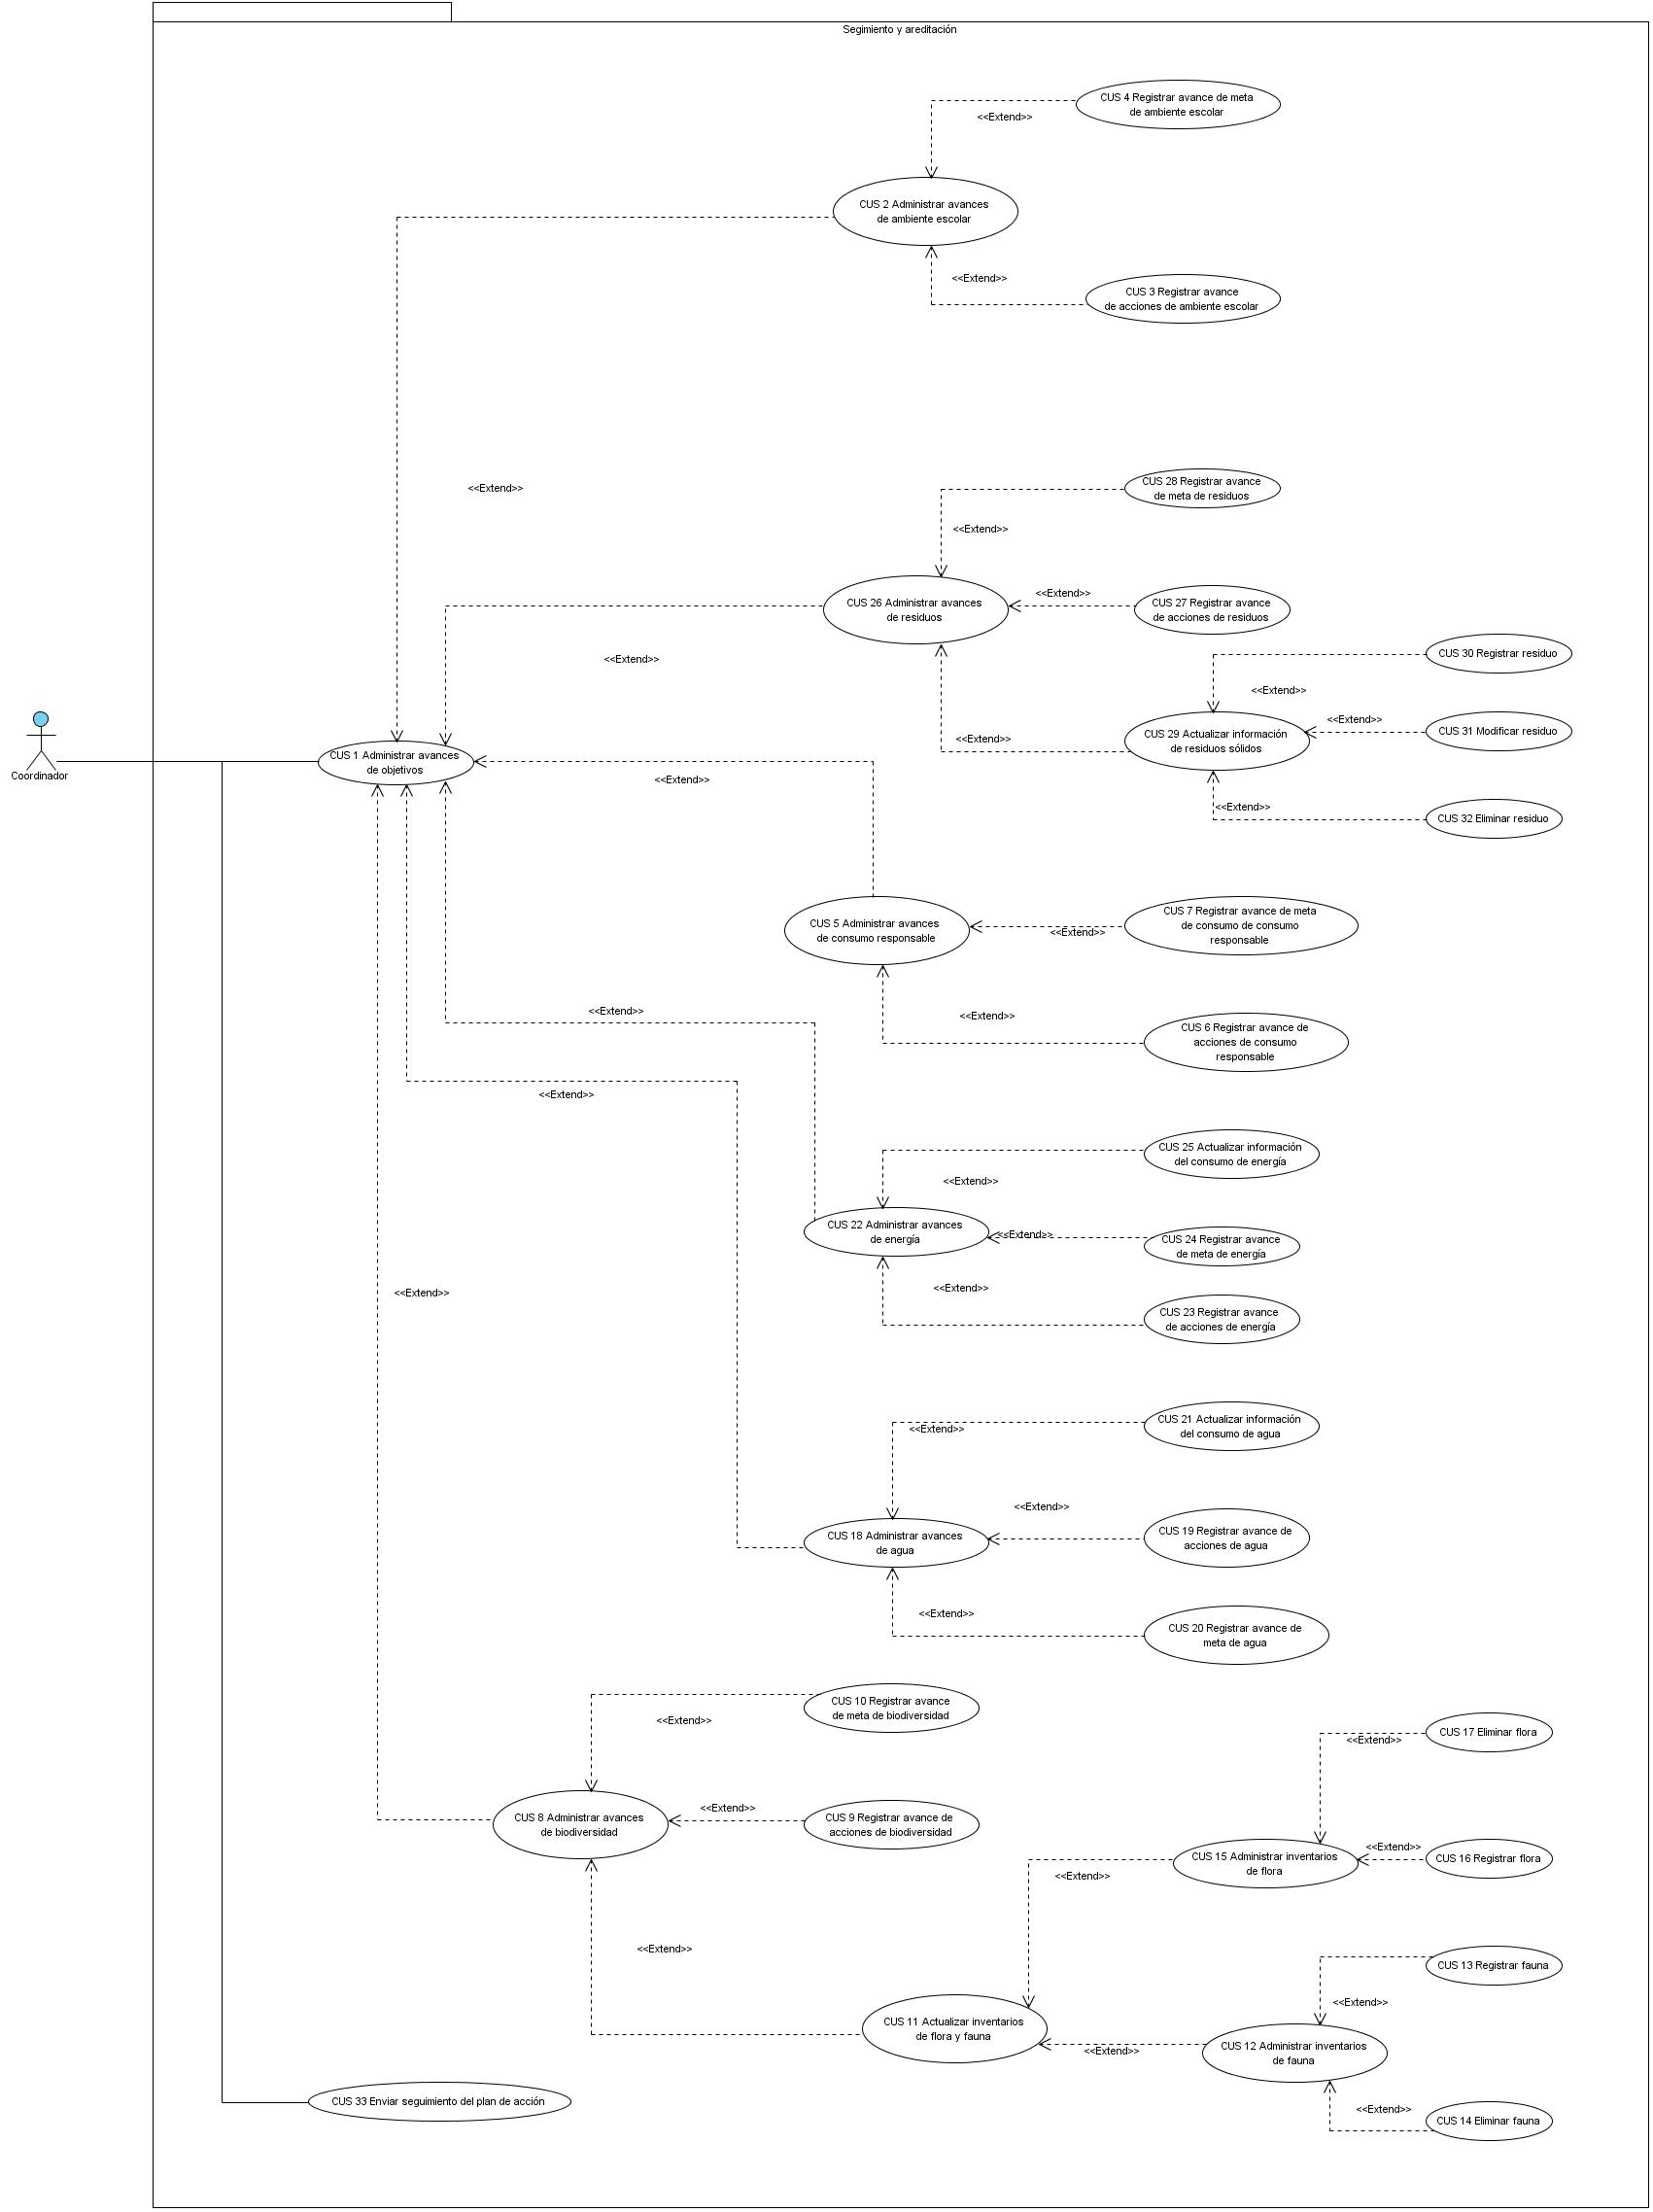
\includegraphics[width=\textwidth]{images/CasosUso/Seguimiento.jpg}}
%    \caption{Diagrama de casos de uso para el módulo de Seguimiento y acreditación.}
%    \label{fig:casosUso:seguimiento}
%    \end{center}
%\end{figure}
%
%\section{Casos de Uso del módulo de Indicadores}
%La figura \ref{fig:casosUso:indicadores} muestra los casos de uso que integran la funcionalidad del módulo de Indicadores, los cuales permiten la visualización de los resultado obtenidos en los indicadores ambientales y de sustententabilidad de la escuela. 
%
%\begin{figure}[h!]
%    \begin{center} 
%        \fbox{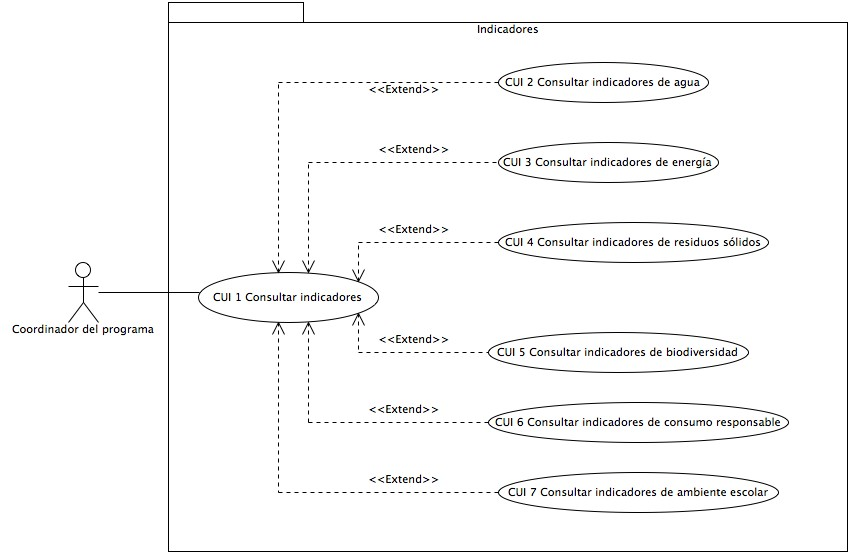
\includegraphics[width=\textwidth]{images/CasosUso/Indicadores.png}}
%    \caption{Diagrama de casos de uso para el módulo de Indicadores.}
%    \label{fig:casosUso:indicadores}
%    \end{center}
%\end{figure}